\section{Recueil d'information et Analyse}

Après avoir défini, avec le client, les grandes lignes du projet il a fallu définir et détailler de manière approfondie toutes les fonctionnalités. Pour ce faire, j'ai décidé de procéder en plusieurs étapes. 

\newpara

\textbf{Premièrement}, plusieurs réunions avec le client ont permis de dégrossir l'ensemble des fonctionnalités. Ainsi, chaque grosse fonctionnalité a été découpée en plus petites, a été détaillée en texte clair et a été contextualisée par rapport à l'ensemble du projet. 
Cette étape fut très importante car elle a permis de concrétiser les besoin du client et de mettre en avant les potentielles difficultés. 

\newpara

\textbf{Dans un second temps}, sur base de l'étape précédente, j'ai transformé le texte claire de chaque fonctionnalité en "user story"\footnote{Une "user story" est, dans le domaine du développement de logiciels, une description simple et structurée d'une fonctionnalité à développer.} Les "user stories" permettent de structurer l'ensemble des fonctionnalité en un format bien défini. Plus d'information quand à la réalisation de celles-ci se trouvent dans le sous-chapitre "User-stories" ci-après. 

\newpara

\textbf{Pour finir}, j'ai analyser et défini avec le client les besoins plus techniques tel que par exemple: 
\begin{itemize}
  \item les liens inter-fonctionnalité
  \item les données à devoir stocker 
  \item les liens entre les différentes données
  \item les implications comptable (au niveau du stock et de la facturation)
  \item une estimation de la quantité de donnée à stocker
  \item les roles des différents utilisateurs
\end{itemize}


\subsection{User-stories}

Comme expliqué précédemment, chaque fonctionnalité à été détaillée sous forme d'une "user story" (US). Dans un but organisationnel, j'ai décidé de grouper chaque US par grande fonctionnalité. Qu'entend-t-on par grande fonctionnalité? Dans le cadre de ce projet, une grande fonctionnalité est un élément fictif faisant référence à l'ensemble des informations et manipulations relatives à un objet du système d'information. A titre d'exemple: la grande fonctionnalité "\textbf{Stock}" regroupe l'ensemble des fonctionnalités permettant de définir la façon dont un utilisateur va pouvoir consulter la quantité restante d'un produit, l'historique d'achat ou de vente d'un produit, la valeur cumulée de tous les produits, ajouter un nouveau produit, etc. 

\newpara

Afin de pouvoir facilement maintenir la multitude d'US, j'ai défini un structure type comportant les éléments suivants :
\begin{enumerate}
  \item Code unique + Titre
  \item Description (du type: \textit{"En tant que X j'aimers Y afin de Z"})
  \item Préconditions
  \item Explication détaillée avec éventuellement des mockups\footnote{\textit{"En informatique, le terme mock-up (qui vient du même mot anglais qui signifie une maquette à l'échelle 1:1) désigne un prototype d'interface utilisateur."}\cite{Mock}}
  \item Critères de validation
\end{enumerate}

\newpage

\subsubsection{Exemple}

\begin{figure}[H]
  \centering
  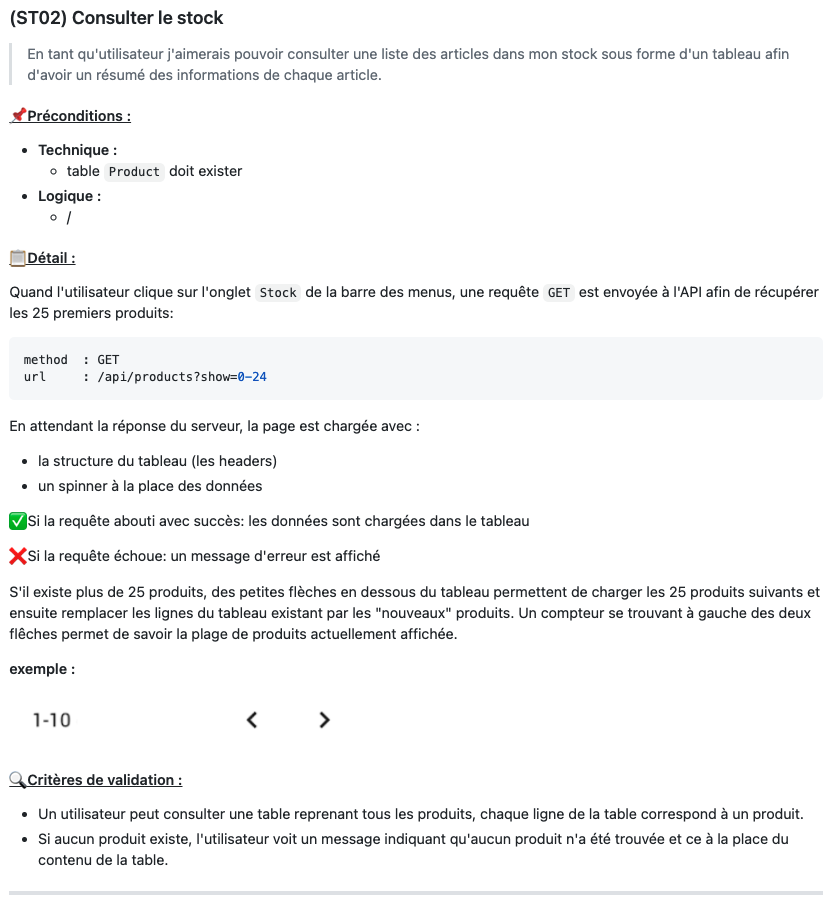
\includegraphics[width=\textwidth]{img/exemple_us.png}
  \caption{Exemple de "user story"}
\end{figure}

L'ensemble des US peuvent-être consultées dans la wiki de la page Github\footnote{\url {https://github.com/MMichotte/SLG_APP/wiki/US_0_home}} de ce projet. 
Notons que toutes les fonctionnalités n'ont pas été transformées en US. J'ai décidé de travailler selon les méthodes de développement "agiles" qui préconisent de ne pas réaliser l'entièreté de l'analyse si cela n'est pas nécessaire au développement. Ma méthodologie de travail est décrite dans un chapitre ultérieur. 

\newpage

\subsubsection{Automatisation Trello}
Une fois une US écrite, je la re-transcrivait sous forme de carte "Trello"\footnote{Trello est un programme des gestion de taches permettant de créer différentes listes et cartes fin d'organiser le travail. Pour plus d'informations voir : \url{https://trello.com}} afin de pouvoir utiliser celle-ci comme base de travail lors de l'implémentation de la fonctionnalité. Cette opération étant fastidieuse et rébarbative, j'ai décidé de développer une petite application en ligne de commande me permettant d'automatiquement générer mes cartes Trello sur base de mes US écrites dans la wiki du Github du projet. 

\newpara

J'ai conçu cette application avec comme objects: 
\begin{enumerate}
  \item imposer une structure d'US
  \item utilisation simple
  \item possibilité d'intégration dans une pipeline de déploiement continu\footnote{Une pipeline de déploiement continu est un ensemble d'actions permettant d'automatiser le déploiement du code depuis un environnement de développer vers un environnement de production. Pour de plus amples informations voir: \url{https://www.redhat.com/fr/topics/devops/what-is-ci-cd}}
  \item ne doit pas avoir d'impact visuel sur les US dans le wiki de github
  \item open-source
\end{enumerate}

\newpara

Bien que la conception de cette application m'ai pris un certain temps, cela est dérisoire par rapport au gain de temps que j'ai pu en tirer. Les fonctionnalités proposée par cette application sont néanmoins encore limités mais le projet étant open-source, tout le monde peut y contribuer. 

\newpara

Une explication plus détaillé n'ayant pas sa place dans ce rapport, elle est disponible sur le Github de ce mini-projet: \url{https://github.com/MMichotte/US-to-TrelloCard}.


\subsection{Base de donnée}
Un bon système d'information repose en grande partie sur la qualité de la base de donnée.  
//TODO 

\begin{sidewaysfigure}
  \centering
  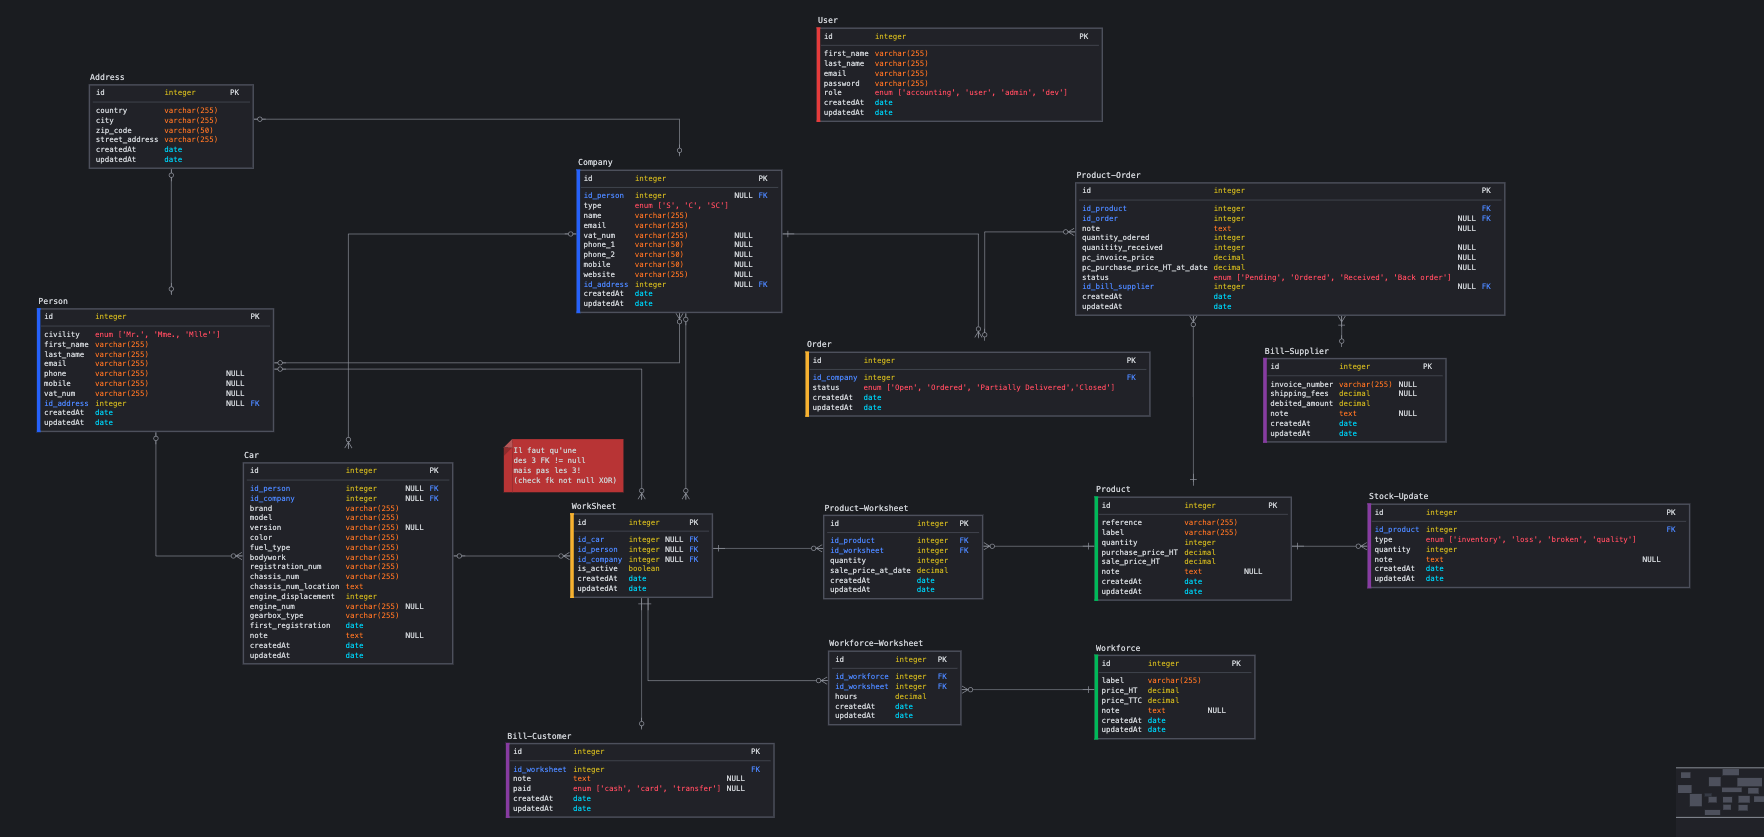
\includegraphics[width=\textwidth]{img/DB-schema.png}
  \caption{Schéma de base de donnée}
\end{sidewaysfigure}